% this file is called up by thesis.tex
% content in this file will be fed into the main document

\chapter{Evaluation of Results} % top level followed by section, subsection
\label{discussionChapter}

% ----------------------- paths to graphics ------------------------

% change according to folder and file names
\ifpdf
    \graphicspath{{7/figures/PNG/}{7/figures/PDF/}{7/figures/}}
\else
    \graphicspath{{7/figures/EPS/}{7/figures/}}
\fi


% ----------------------- contents from here ------------------------

In this chapter the evaluation is performed in three steps: 1) data measured by executing cycle- and application-level experiments is described visually and the plotted graphs are discussed; 2) the model is quantified and updated with values applicable to both processors used in the study; 3) the predicted behaviour of the model is compared to what was measured in a real-life setting.

\section{Deriving Parameters in the Model}

In all of the experiments the results included page faults and interrupt events, which obscured the underlying performance data, as discussed in section \ref{sec:cycle_results}. In figures \ref{Cycle_experiment_dirty_nuim_small} and \ref{Cycle_experiment_dirty_ichec_small}, one would expect to have ``jumps" where written/read data hits the sizes of levels of cache found in the used hardware, but no such events were registered. Instead, abnormalities in other places where they were not expected could be observed, as described in section \ref{sec:cycle_results}. Cache/main memory latency measurements from lmbench suite were used instead. Such results may be used to quantify the model that is described in chapter \ref{chapterModel}.

\subsection{Deriving Latency of Cache and Main Memory}

Because write-back caches are used, latency of reading data is equal to latency of writing data, as described in equation \ref{eq:model5}. The equations \ref{eq:discussion3} and \ref{eq:discussion4} assign measured values of latency to corresponding parameters of the final equations. Values of latency are taken from table \ref{lmbenchTable}. Values are measured in nano-seconds. Cache lines in both processors are 64 B in size. The equation \ref{eq:discussion3} describes latency of accessing cache and main memory in the Xeon 5130. The lines in equation \ref{eq:discussion3} represent:

\begin{enumerate}
  \item Applying a measured with lmbench value of L1 cache latency for the Xeon 5130 to the parameters that represent latency of writing and reading data from/to L1 cache.
  \item Applying a measured with lmbench value of L2 cache latency for the Xeon 5130 to the parameters that represent latency of writing and reading data from/to L2 cache.
  \item Applying a measured with lmbench value of latency of main memory for the Xeon 5130 to the parameters that represent latency of writing and reading data from/to main memory.
  \item Applying measured values of latency for the Xeon 5130 into the cost of writing the amount of memory that can fit into Level 1 cache.
\end{enumerate}

In this equation $lat_{WriteL1\_Xeon5130}$ and $lat_{ReadL1\_Xeon5130}$ are values of latency or writing and reading data from Level 1 cache respectively; $lat_{WriteL2\_Xeon5130}$ and $lat_{ReadL2\_Xeon5130}$ –- Level 2 cache; $lat_{WriteMem\_Xeon5130}$ = $lat_{ReadMem\_Xeon5130}$ –- main memory. $l1w_{Xeon5130}$ and $l1r_{Xeon5130}$ indicate latency of writing and reading data that can fit into L1 cache respectively. The size of \textit{long} (quantum of data exchanged) is 8 bytes on a 64-bit Linux system.

\begin{equation}\label{eq:discussion3}
\begin{split}
1.\; lat_{WriteL1\_Xeon5130} = lat_{ReadL1\_Xeon5130} = 1.5 \\
2.\; lat_{WriteL2\_Xeon5130} = lat_{ReadL2\_Xeon5130} = 7 \\
3.\; lat_{WriteMem\_Xeon5130} = lat_{ReadMem\_Xeon5130} = 100 \\
4.\; l1w_{Xeon5130} = l1r_{Xeon5130} = (n/8 - n/64) * 1.5 \\ 
\end{split}
\end{equation}

The lines in equation \ref{eq:discussion4} represent:

\begin{enumerate}
  \item Applying a measured with lmbench value of L1 cache latency for the Xeon E5-2695 v2 to the parameters that represent latency of writing and reading data from/to L1 cache.
  \item Applying a measured with lmbench value of L2 cache latency for the Xeon E5-2695 v2 to the parameters that represent latency of writing and reading data from/to L2 cache.
  \item Applying a measured with lmbench value of L3 cache latency for the Xeon E5-2695 v2 to the parameters that represent latency of writing and reading data from/to L3 cache.
  \item Applying a measured with lmbench value of latency of main memory for the Xeon E5-2695 v2 to the parameters that represent latency of writing and reading data from/to main memory.
  \item Applying measured values of latency for the Xeon E5-2695 v2 into the cost of writing the amount of memory that can fit into Level 1 cache.
\end{enumerate}

Names of the parameters in equation \ref{eq:discussion4} follow the same convention as in equation \ref{eq:discussion3}. However, in case of equation \ref{eq:discussion4}, because the Xeon E5-2695 v2 also has Level 3 cache, latency of writing and reading data from that level of cache is noted as $lat_{WriteL3\_XeonE5}$ and $lat_{ReadL3\_XeonE5}$ for latency of writing and reading data from Level 3 cache respectively.

\begin{equation}\label{eq:discussion4}
\begin{split}
1.\; lat_{WriteL1\_XeonE5} = lat_{ReadL1\_XeonE5} = 1.25 \\
2.\; lat_{WriteL2\_XeonE5} = lat_{ReadL2\_XeonE5} = 3.75 \\
3.\; lat_{WriteL3\_XeonE5} = lat_{ReadL3\_XeonE5} = 15.5 \\
4.\; lat_{WriteMem\_XeonE5} = lat_{ReadMem\_XeonE5} = 60 \\
5.\; l1w_{XeonE5} = l1r_{XeonE5} = (n/8 - n/64) * 1.25 \\ 
\end{split}
\end{equation}

\subsection{Applying Sizes of Cache and Memory to the Model}

The model contains parameters that indicate sizes of different levels of memory. The lines in equation \ref{eq:discussion5} indicate:

\begin{enumerate}
  \item Size of L1 cache in the Xeon 5130.
  \item Size of L2 cache in the Xeon 5130.
\end{enumerate}

These values are taken from the table \ref{xeonTable}, the sizes are indicated in bytes there. This data is assigned to values $l_{L1\_Xeon5130}$ and $l_{L2\_Xeon5130}$, which indicate sizes of Level 1 and Level 2 caches in the Xeon 5130 respectively.

\begin{equation}\label{eq:discussion5}
\begin{split}
1.\; l_{L1\_Xeon5130} = 32768 \\
2.\; l_{L2\_Xeon5130} = 4194304 \\
\end{split}
\end{equation}

The lines in equation \ref{eq:discussion6} outline:

\begin{enumerate}
  \item Size of L1 cache in the Xeon E5-2695 v2.
  \item Size of L2 cache in the Xeon E5-2695 v2.
  \item Size of L3 cache in the Xeon E5-2695 v2.
\end{enumerate}

$l_{L1\_XeonE5}$, $l_{L2\_XeonE5}$, and $l_{L3\_XeonE5}$ indicate sizes of Level 1, Level2, and Level 3 caches in the Xeon E5-2695 v2.

\begin{equation}\label{eq:discussion6}
\begin{split}
1.\; l_{L1\_XeonE5} = 32768 \\
2.\; l_{L2\_XeonE5} = 262144 \\
3.\; l_{L3\_XeonE5} = 30720000 \\
\end{split}
\end{equation}

\subsection{Deriving Amount of Overhead from the OS}

The amount of overhead from the OS depends on the kind of inter-thread communication that takes place. Data is taken from table \ref{overheadTable}. The lines in equations \ref{eq:discussion7}, \ref{eq:discussion70}, \ref{eq:discussion700}, \ref{eq:discussion7000} represent:

\begin{enumerate}
  \item Overhead from the OS for Type 1 inter-thread communication on the Xeon 5130.
  \item Overhead from the OS for Type 2 inter-thread communication on the Xeon 5130.
  \item Overhead from the OS for Type 3 inter-thread communication on the Xeon 5130.
\end{enumerate}

$Control_{1\_Xeon5130}$ and $Control_{1\_XeonE5}$ indicate how many nano-seconds need to be spent on supplementary processes that take place in Type 1 communication, measured in Experiment 2. Then, $Control_{2\_Xeon5130}$ and $Control_{2\_XeonE5}$ show the overhead from the OS in case of Type 2 communication, it was recorded in Experiment 3. Lastly, $Control_{3\_Xeon5130}$ and $Control_{3\_XeonE5}$ outline the amount of overhead generated by the OS for Type 3 communication, this data was measured by conducting Experiment 4. Each of these parameters represents a sum of overhead caused by exiting the writing thread, transitioning to the reading thread, entering the reading thread, and interference of the OS (e.g. $Control_{exitTh1\_1\_Xeon5130} + Control_{tt\_1\_Xeon5130} + Control_{enterTh2\_1\_Xeon5130} + I_{1\_Xeon5130}$). These figures were measured by performing experiments with no data exchanged between threads. $I_{pf\_min_1\_Xeon5130}$, $I_{pf\_min_2\_Xeon5130}$, and $I_{pf\_min_3\_Xeon5130}$ indicate overhead caused by the occurrence of minor page faults. $I_{pf\_maj_1\_Xeon5130}$, $I_{pf\_maj_2\_Xeon5130}$, and $I_{pf\_maj_3\_Xeon5130}$ point to the impact of major page faults. Equations \ref{eq:discussion7} and \ref{eq:discussion8} show the non-deterministic part of the overhead from the OS, for both processors.

\begin{equation}\label{eq:discussion7}
\begin{split}
1.\; Control_{1\_Xeon5130} = Control_{exitTh1\_1\_Xeon5130} + Control_{tt\_1\_Xeon5130} \\ + Control_{enterTh2\_1\_Xeon5130} + I_{pf\_min_1\_Xeon5130} + I_{pf\_maj_1\_Xeon5130}  = 291408 \\
2.\; Control_{2\_Xeon5130} = Control_{exitTh1\_2\_Xeon5130} + Control_{tt\_2\_Xeon5130} \\ + Control_{enterTh2\_2\_Xeon5130} + I_{pf\_min_2\_Xeon5130} + I_{pf\_maj_2\_Xeon5130}= 297691 \\
3.\; Control_{3\_Xeon5130} = Control_{exitTh1\_3\_Xeon5130} + Control_{tt\_3\_Xeon5130} \\ + Control_{enterTh2\_3\_Xeon5130} + I_{pf\_min_3\_Xeon5130} + I_{pf\_maj_3\_Xeon5130} = 699229 \\
\end{split}
\end{equation}

The lines in equation \ref{eq:discussion8}, \ref{eq:discussion80}, \ref{eq:discussion800}, \ref{eq:discussion8000} represent:

\begin{enumerate}
  \item Overhead from the OS for Type 1 inter-thread communication on the Xeon E5-2695 v2.
  \item Overhead from the OS for Type 2 inter-thread communication on the Xeon E5-2695 v2.
  \item Overhead from the OS for Type 3 inter-thread communication on the Xeon E5-2695 v2.
\end{enumerate}

A similar naming convention is used in the description of overhead for the Xeon E5-2695 v2. Two minor page faults occurred when this data was collected for all three types of inter-thread communication (due to opening files, as discussed in section \ref{OSinterference}). No major page faults, and no interrupts/context switches were detected when this data was measured. Moreover, analysis of results showed that the occurrence of minor and major page faults has stable nature and they can be seen as deterministic data. 

\begin{equation}\label{eq:discussion8}
\begin{split}
1.\; Control_{2\_XeonE5} = Control_{exitTh1\_1\_XeonE5} + Control_{tt\_1\_XeonE5} \\ + Control_{enterTh2\_1\_XeonE5} + I_{pf\_min_1\_XeonE5} + I_{pf\_maj_1\_XeonE5} = 413963 \\
2.\; Control_{3\_XeonE5} = Control_{exitTh1\_2\_XeonE5} + Control_{tt\_2\_XeonE5} \\ + Control_{enterTh2\_2\_XeonE5} + I_{pf\_min_2\_XeonE5} + I_{pf\_maj_2\_XeonE5} = 415428 \\
3.\; Control_{3\_XeonE5} = Control_{exitTh1\_3\_XeonE5} + Control_{tt\_3\_XeonE5} \\ + Control_{enterTh2\_3\_XeonE5} + I_{pf\_min_3\_XeonE5} + I_{pf\_maj_3\_XeonE5} = 1073144 \\
\end{split}
\end{equation}

These are the average readings of overhead. Closer look at results reported in section \ref{results_app_experiments} shows that a number of page faults increases dramatically when memory is written into main memory (refer to appendices \ref{app:app-level-results-2-nuim}, \ref{app:app-level-results-2-ichec}, \ref{app:app-level-results-3-nuim}, \ref{app:app-level-results-3-ichec}, \ref{app:app-level-results-4-nuim}, and \ref{app:app-level-results-4-ichec}). More specifically, in case of the Xeon 5130, instead of two minor page faults per sub-experiment, on average of one page fault occurs per 4094 B of data exchanged via main memory, for all three types of inter-thread communication. Therefore, additional $pf_{Xeon5130} * n / 4094 - (pf_{Xeon5130} * 2)$ need to be added to the total amount of overhead, where $pf_{Xeon5130}$ indicates the duration of one page fault. Duration of two page faults needs to be subtracted, since this information is already taken into account in equation \ref{eq:discussion7}.

Similarly, more interrupts and context switches are generated when main memory is used: on average one interrupt/context switch is registered for each 49727 B of data exchanged. The model can be refined to cater for this behaviour recorded in a real-life setting. Equation \ref{eq:discussion70} shows a refined vision of the amount of overhead from the OS expected on Xeon 5130.

\begin{equation}\label{eq:discussion70}
\begin{split}
1.\; Control_{1\_Xeon5130} = \begin{cases}291408 & 0 \leq n \leq l_{L2\_Xeon5130} \\ 291408 + pf_{Xeon5130} * n / 4094 \\ - (pf_{Xeon5130} * 2) + int_{Xeon5130} * n / 49727 & n > l_{L2\_Xeon5130}\end{cases} \\
2.\; Control_{2\_Xeon5130} = \begin{cases}297691 & 0 \leq n \leq l_{L2\_Xeon5130} \\ 297691 + pf_{Xeon5130} * n / 4094 \\ - (pf_{Xeon5130} * 2) + int_{Xeon5130} * n / 49727 & n > l_{L2\_Xeon5130}\end{cases} \\
3.\; Control_{3\_Xeon5130} = \begin{cases}699229 & 0 \leq n \leq l_{L2\_Xeon5130} \\ 699229 + pf_{Xeon5130} * n / 4094 \\ - (pf_{Xeon5130} * 2) + int_{Xeon5130} * n / 49727 & n > l_{L2\_Xeon5130}\end{cases} \\
\end{split}
\end{equation}

On the Xeon E5-2695 v2, a number of interrupts generated when data is written into main memory is less predictable. On average one page fault per 103107 bytes and one interrupt per 15400020 bytes of data written into main memory occur on that server. Equation \ref{eq:discussion80} outlines a refined vision of the amount of overhead from the OS expected on Xeon E5-2695 v2. Hence, in case of the Xeon E5-2695 v2, additional $pf_{XeonE5} * n / 103107 - (pf_{XeonE5} * 2)$ must be added to the total amount of overhead, where $pf_{XeonE5}$ indicates the duration of one minor page fault on that system. Duration of two page faults needs to be subtracted, it has already been taken into account in equation \ref{eq:discussion8}.

\begin{equation}\label{eq:discussion80}
\begin{split}
1.\; Control_{1\_XeonE5} = \begin{cases}413963 & 0 \leq n \leq l_{L2\_XeonE5} \\ 413963 + pf_{XeonE5} * n / 103107 \\ - (pf_{XeonE5} * 2) + int_{XeonE5} * n / 15400020 & n > l_{L2\_XeonE5}\end{cases} \\
2.\; Control_{2\_XeonE5} = \begin{cases}415428 & 0 \leq n \leq l_{L2\_XeonE5} \\ 415428 + pf_{XeonE5} * n / 103107 \\ - (pf_{XeonE5} * 2) + int_{XeonE5} * n / 15400020 & n > l_{L2\_XeonE5}\end{cases} \\
3.\; Control_{3\_XeonE5} = \begin{cases}1073144 & 0 \leq n \leq l_{L2\_XeonE5} \\ 699229 + pf_{XeonE5} * n / 103107 \\ - (pf_{XeonE5} * 2) + int_{XeonE5} * n / 15400020 & n > l_{L2\_XeonE5}\end{cases} \\
\end{split}
\end{equation}

Section \ref{resultsDurationIntPf} shows results of the experiment that measures the duration of interrupts and page faults on both CPUs. Page faults take different lengths of time. One minor page fault on average takes $pf_{Xeon5130} = 42666$ on the Xeon 5130 and $pf_{XeonE5} = 21733$ on the Xeon E5-2695 v2; the standard division is 2471.3 and 3162.3 respectively. This value is rather large, but it is negligible in a real-world environment.

The duration of interrupts cannot be seen as a constant as well, as was reported in section \ref{resultsDurationIntPf}. One interrupt on average takes $int_{Xeon5130} = 153694$ on the Xeon 5130 and $int_{XeonE5} = 322826$\hl on the Xeon E5-2695 v2; the standard division is 175825.8 and 17043.3 respectively. These numbers also incorporate overhead caused by context switches. This cost is noticeable, but it can be disregarded in a real-world environment. These values are incorporated into equations \ref{eq:discussion700} and \ref{eq:discussion800}. 
\begin{equation}\label{eq:discussion700}
\begin{split}
1.\; Control_{1\_Xeon5130} = \begin{cases}291408 & 0 \leq n \leq l_{L2\_Xeon5130} \\ 291408 + 42666 * n / 4094 \\ - (42666 * 2) + 153694 * n / 49727 & n > l_{L2\_Xeon5130}\end{cases} \\
2.\; Control_{2\_Xeon5130} = \begin{cases}297691 & 0 \leq n \leq l_{L2\_Xeon5130} \\ 297691 + 42666 * n / 4094 \\ - (42666 * 2) + 153694 * n / 49727 & n > l_{L2\_Xeon5130}\end{cases} \\
3.\; Control_{3\_Xeon5130} = \begin{cases}699229 & 0 \leq n \leq l_{L2\_Xeon5130} \\ 699229 + 42666 * n / 4094 \\ - (42666 * 2) + 153694 * n / 49727 & n > l_{L2\_Xeon5130}\end{cases} \\
\end{split}
\end{equation}

\begin{equation}\label{eq:discussion800}
\begin{split}
1.\; Control_{1\_XeonE5} = \begin{cases}413963 & 0 \leq n \leq l_{L2\_XeonE5} \\ 413963 + 21733 * n / 103107 \\ - (21733 * 2) + 322826 * n / 15400020 & n > l_{L2\_XeonE5}\end{cases} \\
2.\; Control_{2\_XeonE5} = \begin{cases}415428 & 0 \leq n \leq l_{L2\_XeonE5} \\ 415428 + 21733 * n / 103107 \\ - (21733 * 2) + 322826 * n / 15400020 & n > l_{L2\_XeonE5}\end{cases} \\
3.\; Control_{3\_XeonE5} = \begin{cases}1073144 & 0 \leq n \leq l_{L2\_XeonE5} \\ 699229 + 21733 * n / 103107 \\ - (21733 * 2) + 322826 * n / 15400020 & n > l_{L2\_XeonE5}\end{cases} \\
\end{split}
\end{equation}

These equations can be simplified. Also, $l_{L2\_Xeon5130}$, and $l_{L3\_XeonE5}$ are given. Equations \ref{eq:discussion7000} and \ref{eq:discussion8000} show the final estimation of the overhead imposed by the OS

\begin{equation}\label{eq:discussion7000}
\begin{split}
Control_{1\_Xeon5130} = \begin{cases}291408 & 0 \leq n \leq 4194304 \\ 206076 + 13.5124 * n & n > 4194304\end{cases} \\
Control_{2\_Xeon5130} = \begin{cases}297691 & 0 \leq n \leq 4194304 \\ 212359 + 13.5124 * n & n > 4194304\end{cases} \\
Control_{3\_Xeon5130} = \begin{cases}699229 & 0 \leq n \leq 4194304 \\ 613897 + 13.5124 * n & n > 4194304\end{cases} \\
\end{split}
\end{equation}

\begin{equation}\label{eq:discussion8000}
\begin{split}
Control_{1\_XeonE5} = \begin{cases}413963 & 0 \leq n \leq 30720000 \\ 370497 + 0.2309 * n & n > 30720000\end{cases} \\
Control_{2\_XeonE5} = \begin{cases}415428 & 0 \leq n \leq 30720000 \\ 371962 +  0.2309 * n & n > 30720000\end{cases} \\
Control_{3\_XeonE5} = \begin{cases}1073144 & 0 \leq n \leq 30720000 \\ 655763 +  0.2309 * n & n > 30720000\end{cases} \\
\end{split}
\end{equation}

One may also notice, that in all cases where caches are used, the first sub-experiment is an outlier: the amounts of generated interrupts and page faults are much higher than what is observed in consequent sub-experiments (refer to appendices \ref{app:app-level-results-2-nuim}, \ref{app:app-level-results-2-ichec}, \ref{app:app-level-results-3-nuim}, \ref{app:app-level-results-3-ichec}, \ref{app:app-level-results-4-nuim}, and \ref{app:app-level-results-4-ichec}). To simplify, since ten sub-experiments are conducted for each experiments, it can be neglected. Additionally, when data is written into cache, the occurrence of one interrupt can be seen in some sub-experiments, but not always. Such non-deterministic behaviour could not be explained, and it is ignored for simplicity.

\subsection{Quantified Model}

Equations \ref{eq:discussion1} and \ref{eq:discussion2} describe the total costs $d_{comm\_Xeon5130}$ and $d_{comm\_XeonE5}$ of communication between two threads that takes place on the Xeon 5130 and the Xeon E5-2695 v2s respectively. These equations take all three kinds of inter-thread communication into account. They are outlined in the taxonomy in section \ref{taxonomy}. A parameter $t$ indicates a type of inter-thread communication described.

\begin{equation}\label{eq:discussion1}
\begin{split}
d_{comm\_Xeon5130} = \begin{cases} n/8 * lat_{WriteL1\_Xeon5130} & n \leq l_{L1\_Xeon5130}\\n * lat_{WriteL2\_Xeon5130} & l_{L1\_Xeon5130} < n \leq l_{L2\_Xeon5130}\\n * lat_{WriteMem\_Xeon5130} & n > l_{L2\_Xeon5130}\end{cases} \\ + \begin{cases}Control_{1\_Xeon5130} & t = 1\\Control_{2\_Xeon5130} & t = 2\\Control_{3\_Xeon5130} & t = 3\end{cases} \\ + \begin{cases}n * lat_{ReadL1\_Xeon5130} & n \leq l_{L1\_Xeon5130}\\n * lat_{ReadL2\_Xeon5130} & l_{L1\_Xeon5130} < n \leq l_{L2\_Xeon5130}\\n * lat_{ReadMem\_Xeon5130} & n > l_{L2\_Xeon5130}\end{cases}
\end{split}
\end{equation}

\begin{equation}\label{eq:discussion2}
\begin{split}
d_{comm\_XeonE5} = \begin{cases} n/8 * lat_{WriteL1\_XeonE5} & n \leq l_{L1\_XeonE5}\\n * lat_{WriteL2\_XeonE5} & l_{L1\_XeonE5} < n \leq l_{L2\_XeonE5}\\n * lat_{WriteL3\_XeonE5} & l_{L2\_XeonE5} < n \leq l_{L3\_XeonE5}\\n * lat_{WriteMem\_XeonE5} & n > l_{L3\_XeonE5}\end{cases} \\ + \begin{cases}Control_{1\_XeonE5} & t = 1\\Control_{2\_XeonE5} & t = 2\\Control_{3\_XeonE5} & t = 3\end{cases} \\ + \begin{cases}n * lat_{ReadL1\_XeonE5} & n \leq l_{L1\_XeonE5}\\n * lat_{ReadL2\_XeonE5} & l_{L1\_XeonE5} < n \leq l_{L2\_XeonE5}\\n * lat_{ReadL3\_XeonE5} & l_{L2\_XeonE5} < n \leq l_{L3\_XeonE5}\\n * lat_{ReadMem\_XeonE5} & n > l_{L3\_XeonE5}\end{cases}
\end{split}
\end{equation}

Finally, by using the equations \ref{eq:discussion3}, \ref{eq:discussion4}, \ref{eq:discussion5}, \ref{eq:discussion6}, \ref{eq:discussion7000}, and \ref{eq:discussion8000}, a number of parameters in the equations \ref{eq:discussion1} and \ref{eq:discussion2} can be replaced by numeric values. After replacement, it becomes possible to derive two final equations \ref{eq:discussion9} and \ref{eq:discussion10} that describe data-sharing in inter-thread communication in two machines powered by the Intel Xeon 5130 and the Intel Xeon E5-2695 v2 processors. Words of type \textit{long} are used in the experiments, so $ns$ is equal to 8 (on both systems). $d_{comm\_Xeon5130}$ and $d_{comm\_XeonE5}$ are measures in nano-seconds.

% \begin{equation}\label{eq:discussion9}
% \begin{split}
% d_{comm\_Xeon5130} = \begin{cases} n * 1.5 & n \leq 32768\\n/64 * 7 + (n - n/64) * 1.5 & 32768 < n \leq 4194304\\n/64 * 100 + (n - n/64) * 1.5 & n > 4194304\end{cases} \\ + \begin{cases}\begin{cases}291408 & 0 \leq n \leq 4194304 \\ 206076 + 13.5124 * n & n > 4194304\end{cases} & t = 1\\\begin{cases}297691 & 0 \leq n \leq 4194304 \\ 212359 + 13.5124 * n & n > 4194304\end{cases} & t = 2\\\begin{cases}699229 & 0 \leq n \leq 4194304 \\ 613897 + 13.5124 * n & n > 4194304\end{cases} & t = 3 \end{cases} \\ + \begin{cases}n * 1.5 & n \leq 32768\\n/64 * 7 + (n - n/64) * 1.5 & 32768 < n \leq 4194304\\n/64 * 100 + (n - n/64) * 1.5 & n > 4194304\end{cases}
% \end{split}
% \end{equation}

\begin{equation}\label{eq:discussion9}
\begin{split}
d_{comm\_Xeon5130} = \begin{cases} n/8 * 1.5 & n \leq 32768\\n/64 * 7 + (n/8 - n/64) * 1.5 & 32768 < n \leq 4194304\\n/64 * 100 + (n/8 - n/64) * 1.5 & n > 4194304\end{cases} \\ + \begin{cases}\begin{cases}291408 & 0 \leq n \leq 4194304 \\ 206076 + 13.5124 * n & n > 4194304\end{cases} & t = 1\\\begin{cases}297691 & 0 \leq n \leq 4194304 \\ 212359 + 13.5124 * n & n > 4194304\end{cases} & t = 2\\\begin{cases}699229 & 0 \leq n \leq 4194304 \\ 613897 + 13.5124 * n & n > 4194304\end{cases} & t = 3 \end{cases} \\ + \begin{cases}n * 1.5 & n \leq 32768\\n/64 * 7 + (n/8 - n/64) * 1.5 & 32768 < n \leq 4194304\\n/64 * 100 + (n/8 - n/64) * 1.5 & n > 4194304\end{cases}
\end{split}
\end{equation}

\begin{equation}\label{eq:discussion10}
\begin{split}
d_{comm\_XeonE5} = \begin{cases} n/8 * 1.25 & n \leq 32768\\n/64 * 3.75 + (n/8 - n/64) * 1.25 & 32768 < n \leq 262144\\n/64 * 15.5 + (n/8 - n/64) * 1.25 & 262144 < n \leq 30720000\\n/64 * 60 + (n/8 - n/64) * 1.25 & n > 30720000\end{cases} \\ + \begin{cases}\begin{cases}413963 & 0 \leq n \leq 30720000 \\ 370497 + 0.2309 * n & n > 30720000\end{cases} & t = 1\\\begin{cases}415428 & 0 \leq n \leq 30720000 \\ 371962 +  0.2108 * n & n > 30720000\end{cases} & t = 2\\\begin{cases}1073144 & 0 \leq n \leq 30720000 \\ 655763 +  0.2108 * n & n > 30720000\end{cases} & t = 3\end{cases} \\ + \begin{cases}n * 1.25 & n \leq 32768\\n/64 * 3.75 + (n/8 - n/64) * 1.25 & 32768 < n \leq 262144\\n/64 * 15.5 + (n/8 - n/64) * 1.25 & 262144 < n \leq 30720000\\n/64 * 60 + (n/8 - n/64) * 1.25 & n > 30720000\end{cases}
\end{split}
\end{equation}

Moreover, equations \ref{eq:discussion9} and \ref{eq:discussion10} can be visualised on a 2D surface. Figures \ref{graph_model_nuim} and \ref{graph_model_ichec} plot the functions described by these two equations. It should be noted that blue and green lines that indicate communication of Type 1 and Type 2 respectively are co-aligned on the graph. The different in overhead caused by the OS in these two cases proved to be insignificant and it has no measurable impact. Figure \ref{graph_model_nuim} shows the delay of $d_{comm\_Xeon5130}$ against buffer size. Throughput ($n / d_{comm\_Xeon5130}$) is plotted to promote understanding of results. Note that the throughput increases with the size of the buffer, until it reaches a maximum value, which is determined by the access time to main memory. The slope of the curve changes as the buffer size reaches the L1 and L2 cache sizes of 32768 B and 4194304 B respectively.

\begin{figure}[ht!]
\centering
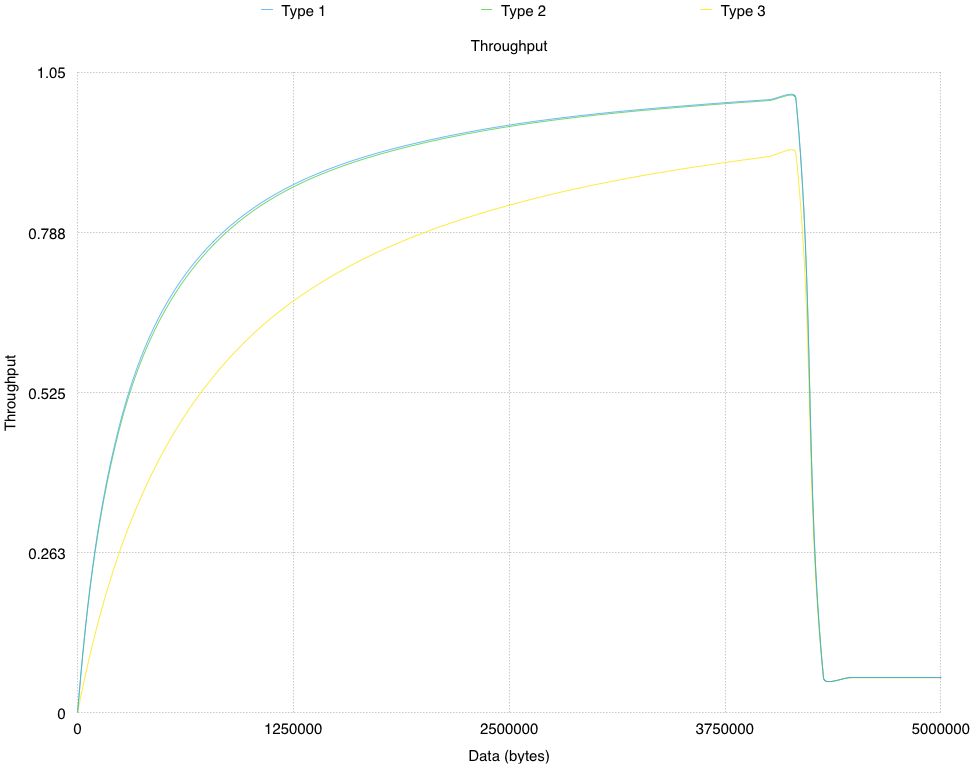
\includegraphics[width=145mm]{7/graph_model_nuim.png}
\caption{Xeon 5130: prediction of throughput of copying data in inter-thread communication}
\label{graph_model_nuim}
\end{figure}

Similarly, figure \ref{graph_model_ichec} renders throughput $n / d_{comm\_XeonE5}$. The throughput increases with the size of the buffer, until it reaches a maximum value, which is determined by the access time to main memory. The slope of the curve changes as the buffer size reaches the L1, L2, and L3 cache sizes of 32768 B, 262144 B and 32000064 B respectively.

\begin{figure}[ht!]
\centering
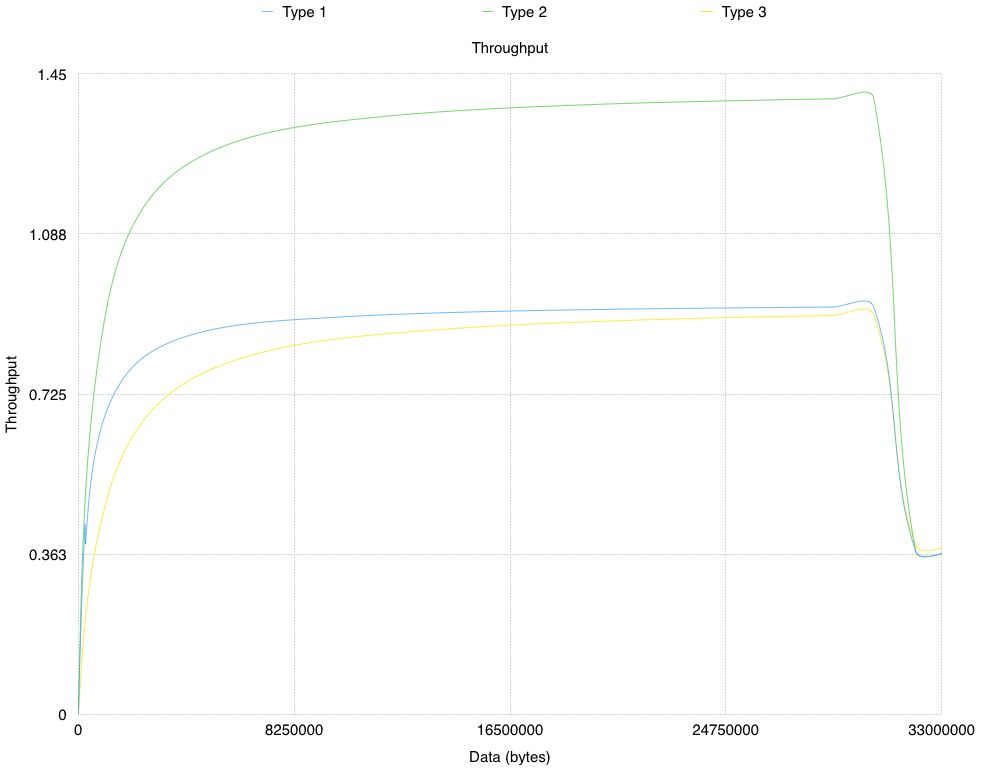
\includegraphics[width=145mm]{7/graph_model_ichec.png}
\caption{Xeon E5-2695 v2: prediction of throughput of copying data in inter-thread communication}
\label{graph_model_ichec}
\end{figure}

This model may be applied to inter-thread communication of any type in any multi-core system with similar to discussed in this project architecture with multiple levels of cache. The equations \ref{eq:discussion9} and \ref{eq:discussion10} and figures \ref{graph_model_nuim} and \ref{graph_model_ichec} presented in this section discuss the applicability of the model to two specific architectures: the Xeon 5130 and the Xeon E5-2695 v2. The next session discusses data that was measured by running the application-level experiments (described in section \ref{app_design}) and compares achieved results with the predictions made by quantifying the model.

\section{Evaluation of the Model}

Data measured through performing Experiment 2, Experiment 3, and Experiment 4 is used to verify the model's predictions of the impact of the cache on inter-thread communication. These experiments outline behaviour of the cache in a real-life setting.

As discussed in section \ref{results_app_experiments}, certain unexpected behaviour was observed when the amount of shared data exceeded 32.0435 MB while executing experiments on both the Xeon 5130 and the Xeon E5-2695 v2. The maximum value on the x-axis in the graph \ref{graph_model_nuim} is 4.75 MB and in case of the graph \ref{graph_model_ichec} it is 31.5MB. Nevertheless, as could be observed by examining the equations \ref{eq:discussion9} and \ref{eq:discussion10}, the function $d_{comm\_Xeon5130}$ has a linear nature for all values of $n$ where $n > 4194304$ (4194304 bytes is the size of the L2 caches). Similarly, the function $d_{comm\_XeonE5}$ also has a linear nature for all values of $n$ where $n > 30720000$ (30720000 bytes is the size of the L3 cache), and all lines on both graphs flatten out after $n$ reaches the size of the last level of cache.

To answer the \textit{RQ4}: cross-examining the graphs \ref{App_experiment_1_throughput_dirty_nuim} and \ref{App_experiment_1_throughput_dirty_ichec} that show throughput for both machines and the figure \ref{graph_model_nuim} and \ref{graph_model_ichec} that plot the equations of the model, shows that the developed model is capable of giving an accurate description of the impact of cache on data-sharing in inter-thread communication. Such model may be used in a cache-aware scheduler. However, there are a number of noticeable differences between the predictions of the model and the real-life results.

\subsection{Accuracy of the Model}

Figures from lmbench incorporate overhead caused by events like interrupts and and page faults. Hence values for latency measured from that benchmarking suite are always higher than (or equal to) the actual readings that can be observed in a laboratory setting where no overhead can be seen. This thesis focuses on the impact of the cache on inter-thread communication in multi-threaded applications that may be seen in the industry. One cannot totally isolate a multi-threaded programme and remove all overhead from the OS. Therefore, results from running experiments in a not fully-isolated environment are of high value. 

The main difference is in the magnitude of throughput. For example, the model shows that exchanging 1280064 bytes of data (1.22 MB) between two threads that reside on different cores of the same chip in the Xeon 5130 should take 1477750 ns, which implies that the value of throughput in this situation should be 0.87. Measuring this situation in the laboratory setting showed that such exchange takes 892488 ns, which is about 40\% times faster than the predicted value, and the reported value of throughput is 1.45.

The model proved to be overly-pessimistic. It could be caused by the inability of the laboratory setting to isolate the experiments from the overhead from the OS. Such advanced technologies as Intel's Advanced Smart Cache may also affect the results (discussed in section \ref{possibleeffects}), but modelling their behaviour is not in the scope of this research. Also, the values of latency that were measured by using lmbench cannot be fully trusted. The tool does not eliminate overhead caused by occurrence of such events as interrupts and page faults. Additionally, this study focuses on the average values of timing measurements. All experiments exhibited extremely large amounts of overhead during their execution, especially during first runs. An attempt to predict the amount of time taken by such events was undertaken, but, the high values of standard deviation reported for both interrupts/context switches and page faults (refer to section \ref{resultsDurationIntPf}) indicate that modelling behaviour of such events is overly-complicated and that it could not be performed in the given laboratory environment. A large decrease of throughput, when data that is shared between two threads exceeds the size of the last level of cache, was observed on both the Xeon 5130 and the Xeon E5-2695 v2. It is an expected result since latency of writing and reading data to/from main memory is much larger than may be observed when caches are used.

The proposed model has a linear or close to linear format for all levels of memory discussed. The plots of data that were achieved by running the experiments have more unpredictable and much more complicated nature, especially in case of the Xeon E5-2695 v2.

\subsection{Implications for Scheduling}

To address the research questions \textit{RQ1} and \textit{RQ2}, the model was able to predict that allocating threads to different cores of the same chip does not yield any noticeable benefits in the writer/reader scenario outlined in the project. The measured result showed that throughput, which can be achieved by scheduling a thread on a different core of the same die, is almost fully identical to what may be measured by pinning both the writing and the reading threads on the same core that has a private Level 1 cache. Similarly, on both graphs \ref{App_experiment_1_throughput_dirty_nuim} and \ref{App_experiment_1_throughput_dirty_ichec}, the lines that represent throughput of communication between threads that are executed by different chips are distinctly ``under" the lines that show throughput achieved during communication of Type 1 and Type 2 nature.

Performance of all three types of scheduling (Type 1: both threads are placed on the same core; Type 2: threads are put on different cores on the same chip; Type 3: threads are scheduled on different chips), as measured in the experiments, can be compared visually. Graphs \ref{thread-placement-nuim} and \ref{thread-placement-ichec} shows the impact of placement of threads for all three cases on both machines. The blue line (Type 1) serves as a base case. Other two lines (green for Type 2 and yellow for Type 3) show the impact relative to the base case, i.e. the differences in latency of scheduling two threads. If the difference is negative, one may conclude that the base case (Type 1) scheduling algorithms has an advantage, it is faster. Both plots feature the moving average trending lines to support understanding of the relations.

\begin{figure}[ht!]
\centering
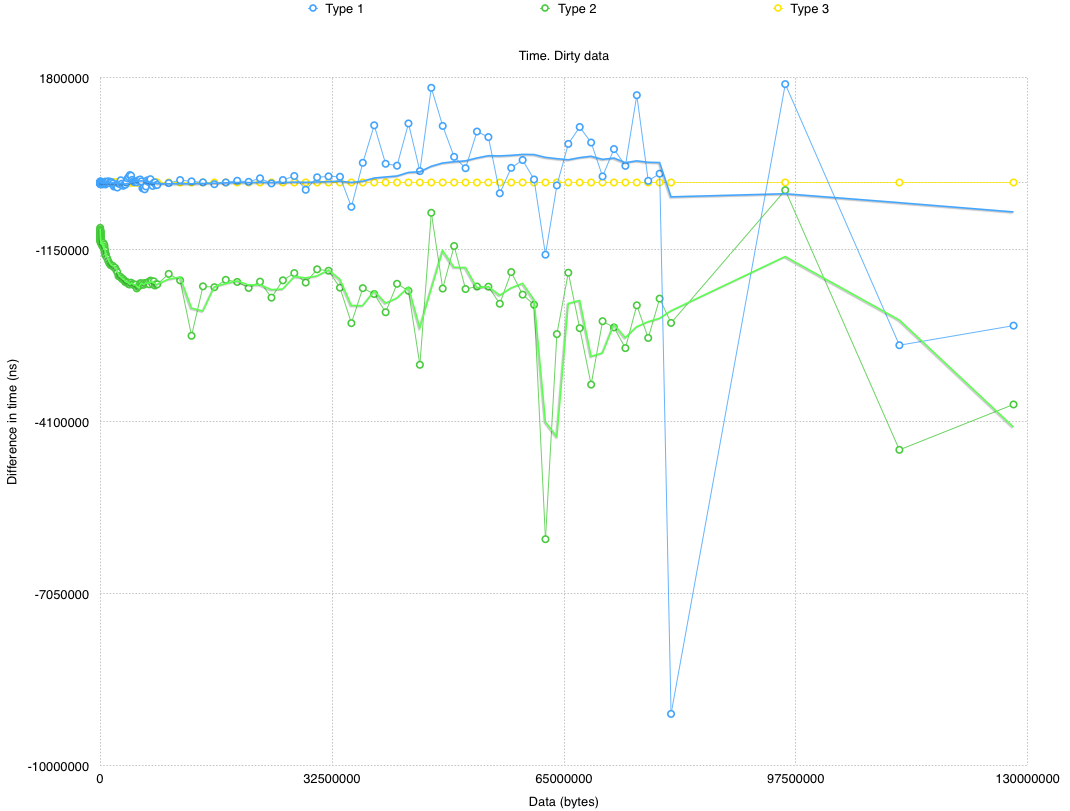
\includegraphics[width=145mm]{7/thread-placement-nuim.png}
\caption{Performance of three ways of scheduling threads, Xeon 5130}
\label{thread-placement-nuim}
\end{figure}

Figure \ref{thread-placement-nuim} shows that the impact of scheduling threads that are engaged in active exchange of data on different cores of the same chip is small (difference: 7.9 $\mu$s or 5\%); in case of placing threads on difference dies, the overhead is large (difference: 1.3 ms or 37\%). Both of these values were measured for the buffer size that is equal to the size of L2 cache in the CPU. There is no significant difference between scheduling threads on the same core and on different cores inside of one chip when less than 30 MB of data is exchanged between threads. When this threshold is reached, placing the receiving thread on a different core results in the increase of the speed of the programme by close. Scheduling the receiving thread on a different core in the same chip for more than around 70 MB of data exchanged between threads leads to the decreased speed of execution. 

Figure \ref{thread-placement-ichec} shows that the same conclusion may be derived: the impact of placing threads on different cores of the same chip in the described scenario is small (difference: 8.9 $\mu$s or 1\%) and scheduling threads on different chips if costly (difference: 1.6 ms or 15\%). Both of these values were measured for the buffer size that is equal to the size of L3 cache in the CPU. Both graphs exhibit positive and negative impact for Type 2 and Type 3 scheduling algorithms: it may be explained by the interference of the OS. A few outliers that are seen on the graphs are also caused by the interference of the Operating System. Examining the figures shows that scheduling both the sending and the receiving threads on different chips has a large impact on the speed of execution. The model gives similar predictions.

\begin{figure}[ht!]
\centering
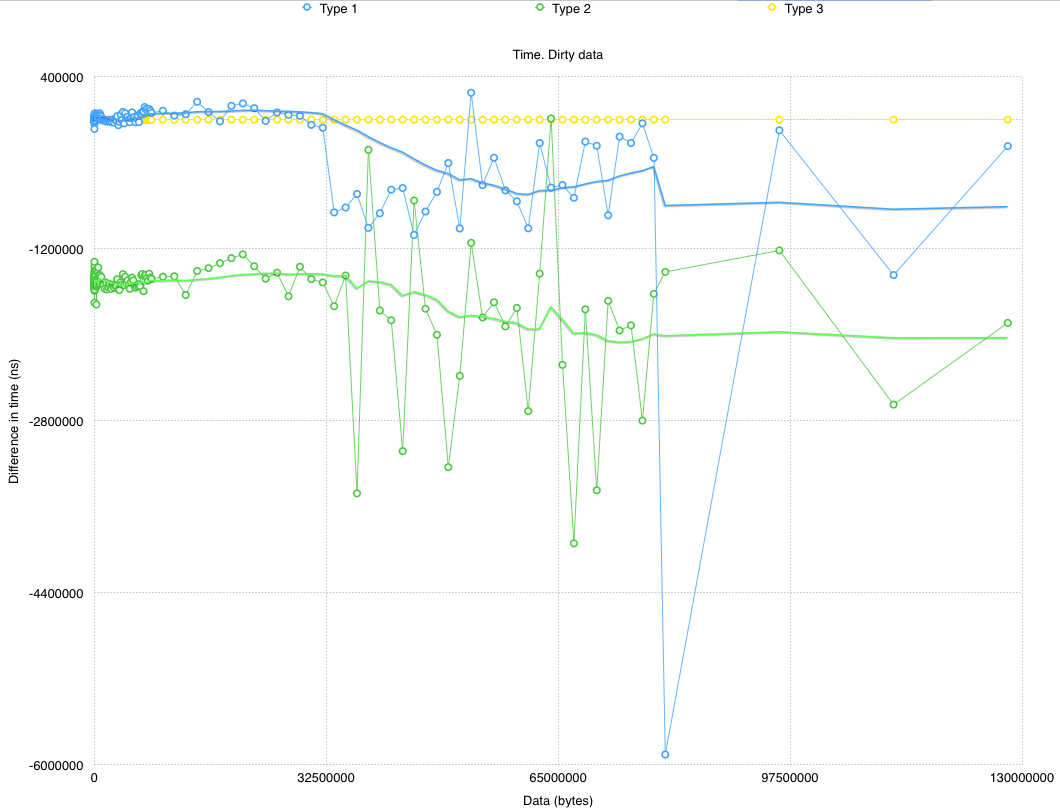
\includegraphics[width=145mm]{7/thread-placement-ichec.png}
\caption{Performance of three ways of scheduling threads, Xeon E5-2695 v2}
\label{thread-placement-ichec}
\end{figure}

It implies that executing threads that share a large amount of data on different processor chips results in decreased performance, and decreases speed of execution. Therefore, \textit{RQ} may be answered: yes, in a situation where a ``sending" and a ``receiving" threads exchange data, a scheduler should take where a receiving thread is scheduled into account.

Cache does have a large impact on the speed of programmes that have threads that are executed by different units of computation (cores or processor chips). To answer the research question \textit{RQ3}, the results received in this study may be used to provide a grounding for creation of a cache-aware scheduler that by using a theoretical model, such as the one proposed in the study, will be able to increase the speed of execution of multi-threaded programmes that have threads that are engaged in inter-thread communication. However, the proposed model needs to be fine-tuned and such aspects of cache as associativeness, differences in latency of reading and writing data and pipelining must be incorporated into the equations. There are a number of possible effects that the model does not cater for.

\section{Possible Effects not Included in the Model}
\label{possibleeffects}

The model focuses on Write-back caches (described in section \ref{cacheLit}). In a Write-through cache, data is mostly read from main memory. A reader in the sender-reader scenario discussed in the thesis would be almost guaranteed to read information, that is exchanged between threads, from main memory, and not from caches. The cache size becomes irrelevant to the speed of a programme.

One technique that is employed in many modern-day computers is data prefetching (described in section \ref{cacheLit}). It is not clear if such technology was enabled on the servers used in the study. Table \ref{prefetching1} shows what the fetch cycle would look like on the Xeon 5130 (with an assumption that the read instructions are pipelined from the i-cache\footnote{Instruction cache.}, and the biggest load comes from d-cache\footnote{Data cache.} reads) if the data cache prefetching is active. Optimum pipleining is assumed.

\begin{table*}[h]
\caption{Fetch cycle with active data prefetching on Xeon 5130}
\begin{tabular}{ll}
Time & Activity                                                                                         \\
0    & CPU read. Cache miss. Start cache line fetch from Level 2 (2 cache lines)                               \\
7.0  & First cache line fetch complete. Read complete (8 bytes) \\
 & Next read instruction starts execution \\
8.5  & Read complete (8 bytes)                                                                          \\
10.0 & Read complete (8 bytes)                                                                          \\
11.5 & Read complete (8 bytes). Cache miss on next read                                                 \\
13.0 & Second cache line complete. Read complete (8 bytes) \\
 & Next read instruction starts execution      \\
14.0 & Read complete (8 B)                                                                              \\
16.0 & Read complete (8 bytes)                                                                          \\
17.5 & Read complete (8 bytes)                                                                         
\end{tabular}
\label{prefetching1}
\end{table*}

Table \ref{prefetching2} shows a fetch cycle for a single cache line. Again, optimum pipleining is assumed.

\begin{table*}[h]
\caption{Single line fetch with no active data prefetching on Xeon 5130}
\begin{tabular}{ll}
Time & Activity                                                                                 \\
0    & CPU read. Cache miss. Start cache line fetch from Level 2 (1 cache line)                        \\
7.0  & Cache line fetch complete. Read complete (8 bytes)\\
 & Next read instruction starts execution \\
8.5  & Read complete (8 bytes)                                                                  \\
10.0 & Read complete (8 bytes)                                                                  \\
11.5 & Read complete (8 bytes). Cache miss on next read                                          \\
18.5 & Cache line fetch complete. Read complete (8 bytes)\\
 & Next read instruction starts execution \\
20.0 & Read complete (8 bytes)                                                                  \\
21.5 & Read complete (8 bytes)                                                                  \\
23.0 & read complete (8 bytes). Cache miss                                                  
\end{tabular}
\label{prefetching2}
\end{table*}

This means that reading 64 bytes (1 cache line) will take 18.5 ns as opposed to 23.0 ns. Hence model can be closer to the real-world results, it is less ``pessimistic". In this case the reported by the model latency is 10 - 20\% smaller than what is measured in the experiments.

Modern Intel processors also utilise the \textit{Advanced Smart Cache} technology \cite{Doweck2006}. This feature allows high bandwidth applications to borrow bandwidth of Level 1 to Level 2 cache from another core with a shared L2 cache. The hardware asks to allocate the full L2 or L3 cache to the application, if the other unit of computation is idle. It enables to reduce the cache miss ratio. Intel reports that it allows to achieve a constant rate of 2 clock-cycles per operation on one cache line \cite{Doweck}. In reality, is is not always a case because of other processes that take place in the system. Table \ref{prefetching3} shows what a fetch cycle would look like in this case (optimum pipelining is assumed).

\begin{table*}[h]
\caption{Fetch cycle when Advanced Smart Cache is enabled on Xeon 5130}
\begin{tabular}{ll}
Time & Activity                                                                                 \\
0    & CPU read. Cache miss. Start cache line fetch from Level 2 (fetching 2 cache \\
 & lines at once using the other core's bandwidth)                   \\
7.0  & Fetch of both cache lines completes. Read complete (8 bytes)\\
 & Next read instruction starts execution \\
8.5  & Read complete (8 bytes)                                                                  \\
10.0 & Read complete (8 bytes)                                                                  \\
11.5 & Read complete (8 bytes)                                          \\
18.5 & Read complete (8 bytes) \\
20.0 & Read complete (8 bytes)                                                                  \\
21.5 & Read complete (8 bytes)                                                                  \\
23.0 & Read complete (8 bytes)                                                  
\end{tabular}
\label{prefetching3}
\end{table*}

Then, instruction pipelining (instruction parallelism), where multiple instructions can be executed at the same time, may influence the behaviour of the model. Because optimum pipelining is assumed in the model, instruction pipelining is unlikely to be a factor in the performance of the model. Parallel instruction execution does not allow faster throughput that is supported by the cache; it is not a significant factor for the accuracy of the model. The cache bus may also be an additional factor.

\section{Survey of Similar Results}

A number of similar to was is described in the thesis experiments are reported in an article \cite{Molka2009a}. It investigates the latency of cache on a Nehelam architecture\footnote{A 45--nm architecture that was used by Intel during 2008 -- 2011.}. The finding reported in the article cannot be used to compare what is descried in this thesis since the Woodcrest\footnote{A 65--nm architecture that was used by Intel during 2006 -- 2008.} and Ivy Bridge\footnote{A 22--nm architecture that is currently used by Intel.} architectures are utilised in the experimental environment. Authors of \cite{KentMilfeldKazushigeGotoAviPurkayastha2007} also discuss results of a number of benchmarks that evaluate speed of multi-threaded programmes. They focus on the changes in the architecture of CPUs that are caused by increasing clock speed and usage of multiple cores. Both shared and independent cache systems are evaluated. It was reported that the locality of data in independent cache systems has to be ensured by operations that can cost as many as 5000 clock cycles each. It is a very large overhead for such operation.

Data that is reported from the experiments has a dependency on the figures of cache latency measured with lmbench. As described in section \ref{results_lmbench}, such numbers could not be fully trusted, due to the closed nature and the age of the benchmark. A report of similar measurements performed with this tool may be found in \cite{Prakash2007}. The paper reports memory-load latency for the Intel Core 2 Duo E6400 processor. Despite the difference in the architectures, the curves of graphs reported in the publication can be related to the findings in this project. The findings are similar to what is reported in this thesis.

Modelling behaviour of cache is a difficult undertaking \cite{Shen2000,Putigny2014}. The paper \cite{Putigny2014} discusses that automatic hardware mechanisms (such as prefetchers and cache coherence protocols) improve performance, but they also make modelling of the impact of the cache more difficult. Many sources provide rules for compiler optimization through analysing data locality by means of computing stack distances\footnote{\textit{Stack distance} -- a depth of a stack, that a reference needs to be extracted from.} \cite{Vera2004,Cacaval2003}, such analysis is easier to conduct, since behaviour of the aforementioned optimisation techniques can be ignored, but it yields limited conclusions.

% ---------------------------------------------------------------------------
% ----------------------- end of thesis sub-document ------------------------
% ---------------------------------------------------------------------------